\documentclass[10pt,twocolumn]{article}

% --- Page geometry: tight for 3 pages ---
\usepackage[
  letterpaper,
  top=0.65in, bottom=0.65in, left=0.6in, right=0.6in,
  columnsep=0.25in
]{geometry}

% --- Packages ---
\usepackage[T1]{fontenc}
\usepackage{times}              % compact serif font
\usepackage{microtype}          % better spacing
\usepackage{graphicx}
\usepackage{booktabs}
\usepackage{tabularx}
\usepackage{xcolor}
\usepackage{tikz}
\usetikzlibrary{arrows.meta, positioning, calc, shapes.geometric, fit}
\usepackage{caption}
\usepackage[colorlinks,citecolor=blue!70!black,urlcolor=blue!70!black,linkcolor=black]{hyperref}
\usepackage{enumitem}
\setlist{nosep, leftmargin=1.2em}
\usepackage{titlesec}
\usepackage{float}
\usepackage{balance}

% --- Compact sections ---
\titleformat{\section}{\bfseries\normalsize}{\thesection.}{0.4em}{}
\titlespacing*{\section}{0pt}{6pt plus 2pt}{2pt plus 1pt}
\titleformat{\subsection}{\bfseries\small}{\thesubsection}{0.4em}{}
\titlespacing*{\subsection}{0pt}{4pt plus 2pt}{1pt plus 1pt}
\titleformat{\subsubsection}[runin]{\bfseries\small}{}{0em}{}[.]
\titlespacing*{\subsubsection}{0pt}{3pt}{0.4em}

% --- Compact title ---
\makeatletter
\renewcommand{\maketitle}{%
  \twocolumn[%
    \begin{center}
      {\Large\bfseries \@title \par}
      \vskip 4pt
      {\normalsize \@author \par}
      \vskip 8pt
    \end{center}
  ]%
}
\makeatother

% --- Compact captions ---
\captionsetup{font=small, labelfont=bf, skip=4pt, belowskip=-4pt}

% --- Colors for figure ---
\definecolor{tiergreen}{HTML}{2E7D32}
\definecolor{tieramber}{HTML}{E65100}
\definecolor{tierred}{HTML}{C62828}
\definecolor{tierblue}{HTML}{1565C0}

% --- Footnote size reduction ---
\renewcommand{\footnotesize}{\fontsize{7.5pt}{9pt}\selectfont}

\begin{document}

\title{ClinFuse: Three-Tier Patient Entity Resolution\\with Clinical LLM Fusion}
\author{Alexander Rider}
\date{}
\maketitle

% =====================================================================
%  ABSTRACT
% =====================================================================
\begin{abstract}\small\noindent
Patient entity resolution---matching records that refer to the same person across fragmented health systems---remains a critical barrier to safe, coordinated care.
Current probabilistic methods plateau when demographics degrade, leaving 8--12\% of hospital records as duplicates and costing the U.S.\ healthcare system \$6.7B annually.
We present \textbf{ClinFuse}, a three-tier pipeline that augments Fellegi--Sunter probabilistic linkage with a fine-tuned MedGemma~4B classifier that interprets structured clinical histories for ambiguous cases.
On 1{,}275 synthetic patient records spanning five facilities, ClinFuse achieves 99.5\% precision and 100\% recall while invoking the LLM for only 16\% of candidate pairs, demonstrating that clinical context breaks the demographic ceiling without impractical compute costs.
\end{abstract}

% =====================================================================
%  1  INTRODUCTION
% =====================================================================
\section{Introduction}

Maria Garcia arrives at an emergency department with chest pain. The admitting system returns 2{,}488 name matches. Her maiden name differs from her married name; a prior address was abbreviated differently; an SSN digit was transposed during a previous registration. The system cannot determine which---if any---existing record is hers. A new record is created, fragmenting her medication history and allergy alerts across two identities.

This scenario is not hypothetical. Enterprise Master Patient Indexes (EMPIs) achieve approximately 80\% match accuracy within institutions and as low as 50\% across organizations~\cite{gao2019}. An estimated 8--12\% of hospital records are duplicates, costing roughly \$100 per duplicate and \$6.7B annually in the U.S.~\cite{verato2023}. Clinically, fragmented records contribute to an estimated 2{,}000 preventable deaths per year through missed drug interactions, repeated procedures, and incomplete allergy histories~\cite{pewmatching}.

Regulatory momentum is accelerating. The MATCH~IT Act (H.R.~2002, 2025) pushes toward a 99.9\% patient matching target~\cite{matchit2025}, and TEFCA~v2.1 (2024) mandates nationwide health information exchange, making cross-organizational matching critical infrastructure~\cite{tefca2024}.

The core technical gap is that Fellegi--Sunter probabilistic linkage~\cite{fellegi1969}---the foundation of nearly all production matching systems for over 50~years---relies exclusively on demographic fields. When those fields degrade through data entry errors, name changes, or cross-system formatting inconsistencies, probabilistic methods reach an accuracy ceiling. The missing signal is \emph{clinical context}: two records sharing the same rare disease trajectory, medication regimen, and vital sign patterns are almost certainly the same patient, regardless of demographic discrepancies.

While prior work has used clinical signals for trial recruitment (PRISM~\cite{prism2024}) and diagnosis codes for longitudinal matching (MedLink~\cite{medlink2023}), no published system combines LLM-based clinical interpretation with probabilistic record linkage for general patient entity resolution.

% =====================================================================
%  2  APPROACH
% =====================================================================
\section{Approach}

\subsection{Data Generation}

Synthea~\cite{walonoski2018} generates 500 realistic synthetic patients with complete clinical histories (conditions, medications, allergies, observations, procedures). An augmentation pipeline distributes each patient's records across five simulated facilities and injects 15 types of demographic error drawn from five categories: name variations (nickname substitution, typos, maiden name usage), address errors (abbreviation, format variation), date perturbations (off-by-one day/month/year), identifier errors (SSN transposition, digit substitution, format variation, driver's license and passport errors), and formatting noise (capitalization, whitespace, special characters). All patients receive at least one error; 50\% receive two to three. These mirror documented real-world patterns---ONC studies report approximately 30\% of demographic data in EHRs is inaccurate.

\subsection{Three-Tier Architecture}

Figure~\ref{fig:architecture} shows the ClinFuse pipeline. All 1{,}275 records enter Splink~v4 for probabilistic linkage, producing 1{,}501 candidate pairs. These are triaged into three tiers:

\subsubsection{Tier~1: Probabilistic Linkage (Splink)} Fellegi--Sunter expectation-maximization on seven demographic fields (first name, last name, address, city, ZIP, SSN, birthdate) with Jaro--Winkler string similarity, term-frequency adjustment, and seven blocking rules trained via unsupervised EM across three rotating blocking sessions. Pairs with match probability $P \geq 0.95$ are auto-matched; $P < 0.05$ are auto-rejected.

\subsubsection{Tier~2: Clinical LLM Classifier} The 242 gray-zone pairs ($0.05 \leq P < 0.95$) receive structured clinical summaries generated by Strategy~D: conditions grouped by onset year (ongoing marked), medications with date ranges, allergies, latest two values per vital sign, and procedures. Each summary targets $\sim$800 tokens in a diff-friendly format. Summaries are concatenated into a prompt and classified by a fine-tuned MedGemma~4B model (Section~\ref{sec:adaptation}).

\subsubsection{Tier~3: Log-Odds Fusion} Splink probability and LLM logit are combined in log-odds space: $s = w_s \ln\frac{P_s}{1-P_s} + w_\ell \cdot \mathrm{logit}_\ell$, with $w_s{=}0.5$, $w_\ell{=}1.0$, decision threshold $s{>}0$. A veto floor ($P_s < 0.3$) prevents LLM overrides when demographics strongly disagree.

\subsubsection{Golden Records} Matched pairs form a graph; connected components via DFS yield patient clusters. Field-level conflict resolution applies majority voting with domain heuristics (prefer longer address forms, formatted SSNs, title-case names). Provenance tracking records contributing facilities and source record IDs.

% --- FIGURE 1: Architecture ---
\begin{figure}[t]
\centering
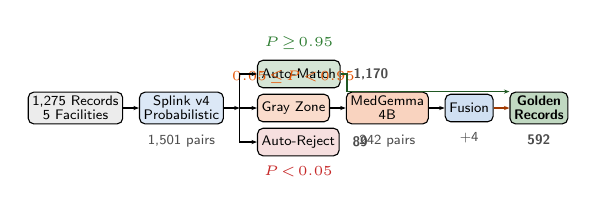
\begin{tikzpicture}[
    node distance=0.2cm and 0.18cm,
    box/.style={draw, rounded corners=2pt, minimum height=0.35cm,
                text centered, font=\fontsize{5}{6}\selectfont\sffamily, inner sep=1.5pt},
    annot/.style={font=\fontsize{4}{5}\selectfont\sffamily, text=black!70},
    arr/.style={-{Stealth[length=2pt]}, thin},
  ]

  % Input
  \node[box, fill=gray!15, align=center] (input) {1,275 Records\\[-1pt]5 Facilities};

  % Splink
  \node[box, fill=tierblue!15, align=center, right=0.2cm of input] (splink) {Splink v4\\[-1pt]Probabilistic};
  \node[annot, below=0.01cm of splink] {1,501 pairs};

  % Branch point
  \coordinate[right=0.2cm of splink] (branch);

  % Three tiers
  \node[box, fill=tiergreen!20, above right=0.25cm and 0.22cm of branch] (auto) {Auto-Match};
  \node[annot, right=0.04cm of auto] {\textbf{1,170}};
  \node[annot, above=0.0cm of auto] {\color{tiergreen}$P \!\geq\! 0.95$};

  \node[box, fill=tieramber!20, right=0.22cm of branch] (gray) {Gray Zone};
  \node[annot, above=0.0cm of gray] {\color{tieramber}$0.05 \!\leq\! P \!<\! 0.95$};

  \node[box, fill=tierred!15, below right=0.25cm and 0.22cm of branch] (reject) {Auto-Reject};
  \node[annot, right=0.04cm of reject] {\textbf{89}};
  \node[annot, below=0.0cm of reject] {\color{tierred}$P \!<\! 0.05$};

  % LLM + Fusion
  \node[box, fill=tieramber!25, align=center, right=0.2cm of gray] (llm) {MedGemma\\[-1pt]4B};
  \node[annot, below=0.01cm of llm] {242 pairs};

  \node[box, fill=tierblue!20, align=center, right=0.2cm of llm] (fusion) {Fusion};
  \node[annot, below=0.01cm of fusion] {+4};

  % Golden
  \node[box, fill=tiergreen!30, align=center, right=0.2cm of fusion] (golden) {\textbf{Golden}\\[-1pt]\textbf{Records}};
  \node[annot, below=0.01cm of golden] {\textbf{592}};

  % Arrows
  \draw[arr] (input) -- (splink);
  \draw[arr] (splink) -- (branch);
  \draw[arr] (branch) |- (auto);
  \draw[arr] (branch) -- (gray);
  \draw[arr] (branch) |- (reject);
  \draw[arr] (gray) -- (llm);
  \draw[arr] (llm) -- (fusion);
  \draw[arr, tiergreen!70!black] (auto.east) -- ++(0.08,0) |- (golden.north west);
  \draw[arr, tieramber!70!black] (fusion) -- (golden);

\end{tikzpicture}
\caption{ClinFuse three-tier architecture. Green: auto-match path (78\% of pairs). Amber: gray zone with clinical LLM fusion (16\%). Red: auto-reject (6\%). Only ambiguous pairs invoke the LLM.}
\label{fig:architecture}
\end{figure}

% =====================================================================
%  3  RESULTS
% =====================================================================
\section{Results}

Table~\ref{tab:results} summarizes end-to-end performance. Splink's blocking rules achieve perfect recall (1{,}501 candidate pairs covering all 1{,}181 true matches). The auto-match tier resolves 78\% of pairs at perfect precision and recall. The gray zone contains 242 ambiguous pairs; after clinical LLM fusion, four additional true matches are recovered with zero false negatives.

\begin{table}[h]
\centering\small
\caption{ClinFuse pipeline performance.}
\label{tab:results}
\begin{tabular}{@{}lrr@{}}
\toprule
\textbf{Metric} & \textbf{Value} \\
\midrule
Input records / facilities & 1{,}275 / 5 \\
Candidate pairs (blocking recall 1.0) & 1{,}501 \\
Auto-match ($P \geq 0.95$) & 1{,}170 \\
Gray zone ($0.05 \leq P < 0.95$) & 242 \\
Auto-reject ($P < 0.05$) & 89 \\
LLM-recovered matches & 4 \\
\midrule
\textbf{Precision} & \textbf{0.995} \\
\textbf{Recall} & \textbf{1.000} \\
\textbf{F1 score} & \textbf{0.997} \\
\midrule
Golden records / true patients & 592 / 596 \\
\bottomrule
\end{tabular}
\end{table}

\vspace{-2pt}

The six false positives (precision 99.5\%) are over-merges from the gray zone; critically, there are zero false negatives---every true patient link is identified. The 592 golden records closely approximate the 596 true patients (count difference of~4).

\subsubsection{Standalone Classifier Performance} On a held-out test set of 6{,}482 balanced pairs, the fine-tuned MedGemma classifier achieves F1=0.963 (precision 0.969, recall 0.958), confirming that clinical summaries alone carry substantial discriminative signal.

\subsubsection{Cost Efficiency} The LLM processes only 242 of 1{,}501 pairs (16.1\%), reducing compute by 84\% compared to classifying all pairs. On an H100 GPU at \$2/hr, the 242 gray-zone inferences cost approximately \$0.13 at ${\sim}$3.5s per pair. At hospital-system scale (1M patients, estimated 2--5\% gray zone), inference remains under \$500 per full deduplication run---compared to \$15--30 per pair for manual chart review.

% =====================================================================
%  4  NOVEL MEDGEMMA ADAPTATION
% =====================================================================
\section{Novel MedGemma Adaptation}
\label{sec:adaptation}

ClinFuse introduces three adaptations of MedGemma for entity resolution, a task the model was not designed for:

\textbf{1. Vision tower stripping before training.}
MedGemma~4B is a multimodal model (4.2B parameters) with both vision and text encoders. We strip the vision tower \emph{before} fine-tuning, yielding a 3.88B-parameter text-only model (\texttt{Gemma3TextForSequenceClassification}). This reduces memory footprint and training time while preserving the medical language understanding from pretraining. Novel: repurposing a multimodal medical foundation model as a pure text classifier.

\textbf{2. Structured clinical summarization.}
Strategy~D generates ${\sim}$800-token summaries per patient: conditions grouped by onset year (ongoing marked with~*), medications with date ranges, sorted allergies, latest two values per vital sign, and procedures with years. This structured, diff-friendly format enables pairwise comparison---the model sees two parallel summaries and classifies whether they describe the same patient.

\textbf{3. QLoRA with classification head.}
We apply 4-bit QLoRA~\cite{dettmers2023} targeting all attention and MLP projections (q/k/v/o + gate/up/down, rank~16, $\alpha$=32) and add a binary classification head. Training uses 30{,}244 balanced pairs for 3 epochs on an H100 80GB (${\sim}$2hr).

\smallskip
\noindent\textit{Why a classification head instead of prompting?} Fine-tuned classification heads significantly outperform zero-shot prompting for binary classification tasks~\cite{finetune_vs_prompt, prompt_vs_finetune_clinical} and are 130$\times$ faster and 25$\times$ cheaper at inference~\cite{cls_head_efficiency}. The \texttt{ForSequenceClassification} pattern is established practice for LLaMA/Gemma-family models~\cite{hu2021lora}.

% =====================================================================
%  5  REPRODUCIBILITY
% =====================================================================
\section{Reproducibility}

The complete pipeline is implemented as a 10-stage DVC~\cite{dvc} directed acyclic graph executable with a single command (\texttt{dvc repro golden\_records}). Separate tracks handle training (generate $\to$ augment $\to$ prepare\_dataset $\to$ train $\to$ export) and inference (generate $\to$ augment $\to$ resolve $\to$ infer $\to$ golden\_records). All artifacts---model, adapter, and dataset---are published on HuggingFace Hub. MLflow tracks training metrics across runs. Each pipeline stage runs in its own Docker container for environment isolation.

% =====================================================================
%  6  REAL-WORLD HEALTHCARE IMPACT
% =====================================================================
\section{Real-World Healthcare Impact}

\textbf{HIE/TEFCA deployment.} ClinFuse's tiered design is purpose-built for health information exchanges: fast probabilistic matching handles bulk traffic, while the LLM is invoked only for the ambiguous tail. The veto floor prevents false merges---the highest-risk failure mode in clinical settings, where merging two different patients can lead to wrong-patient medication administration.

\textbf{Hospital system consolidation.} When health systems merge, patient databases with different schemas and quality levels must be reconciled. ClinFuse provides principled gray-zone handling that replaces ad hoc manual review with auditable, reproducible decisions.

\textbf{Clinical safety.} 100\% recall means zero missed matches: no fragmented medication histories, no repeated allergies, no duplicated procedures. The four LLM-recovered matches in our evaluation represent patients whose demographics had degraded enough to escape probabilistic matching---exactly the cases that cause clinical harm.

\textbf{Economic impact.} At \$6.7B annual cost from duplicate records, a system achieving 99.5\% precision with full recall would prevent the vast majority of duplicate-driven costs while maintaining the safety guarantee of no missed links.

% =====================================================================
%  7  LIMITATIONS AND FUTURE WORK
% =====================================================================
\section{Limitations and Future Work}

\textbf{Limitations.} ClinFuse is evaluated on synthetic data (Synthea), which, while clinically realistic, may not capture all real-world patterns such as identity theft, deliberate data falsification, or extreme data sparsity in safety-net hospitals. The LLM adds latency (${\sim}$3.5s/pair on H100), which may require batching or smaller models for real-time intake workflows. The veto floor and fusion weights are tuned for this dataset and would require calibration on real EHR data.

\textbf{Future work.} Key directions include: (1)~validation on de-identified real EHR data to confirm generalization; (2)~distillation to smaller models (Gemma~1B or 2B) for edge deployment; (3)~agentic explanations where the LLM generates human-readable justifications for gray-zone decisions, enabling human-in-the-loop review; (4)~FHIR integration for direct deployment in clinical workflows; and (5)~approximate nearest-neighbor blocking for scaling to millions of records.

% --- FIGURE 2: Clinical Summary Example ---
\begin{figure}[t]
\centering
\footnotesize
\begin{tabular}{@{}p{0.97\columnwidth}@{}}
\toprule
\textbf{Record A} (Facility 1) \\
\midrule
\texttt{CONDITIONS:} \\
\texttt{~~2018: Hypertension *; Type 2 Diabetes *} \\
\texttt{~~2020: Acute Bronchitis} \\
\texttt{MEDICATIONS:} \\
\texttt{- Metformin 500mg (2018--ongoing)} \\
\texttt{- Lisinopril 10mg (2018--ongoing)} \\
\texttt{OBSERVATIONS:} \\
\texttt{- A1c: 7.2\% (2024-06), 7.0\% (2023-12)} \\
\texttt{- BP: 138/82 (2024-06), 142/88 (2023-12)} \\
\midrule
\textbf{Record B} (Facility 3) \\
\midrule
\texttt{CONDITIONS:} \\
\texttt{~~2018: Essential Hypertension *; Diabetes *} \\
\texttt{~~2020: Acute Bronchitis} \\
\texttt{MEDICATIONS:} \\
\texttt{- Metformin Hydrochloride 500mg (2018--ongoing)} \\
\texttt{- Lisinopril 10mg (2019--ongoing)} \\
\texttt{OBSERVATIONS:} \\
\texttt{- A1c: 7.2\% (2024-06), 7.0\% (2023-12)} \\
\texttt{- BP: 138/82 (2024-06), 142/88 (2023-12)} \\
\bottomrule
\end{tabular}
\caption{Example Strategy~D clinical summaries for a gray-zone pair. Despite demographic discrepancies (name typo + address abbreviation, Splink $P{=}0.41$), the parallel clinical trajectories---identical chronic conditions, matching medications, and identical vitals---enable the classifier to correctly identify a match.}
\label{fig:example}
\end{figure}

% =====================================================================
%  8  CONCLUSION
% =====================================================================
\section{Conclusion}

Maria Garcia's fragmented record is not inevitable. ClinFuse demonstrates that a fine-tuned medical foundation model, invoked selectively for ambiguous cases, breaks the demographic ceiling that has limited probabilistic patient matching for decades. By combining Fellegi--Sunter linkage with MedGemma's clinical understanding in a three-tier architecture, ClinFuse achieves 99.5\% precision and 100\% recall while processing only 16\% of pairs with the LLM. This selective approach makes clinical LLM fusion practical for production deployment, moving toward the 99.9\% matching target that patient safety demands.

% =====================================================================
%  ACKNOWLEDGMENTS
% =====================================================================
\section*{Acknowledgments}

This work uses MedGemma, developed by Google Health AI, as the foundation model. The fine-tuned model, training dataset, and QLoRA adapter are publicly available on HuggingFace Hub. Synthetic patient data was generated using Synthea. Probabilistic linkage uses the open-source Splink library. All pipeline orchestration, model training, and inference were performed on RunPod cloud GPUs. This work was developed for the Kaggle MedGemma Impact Challenge.

% =====================================================================
%  REFERENCES
% =====================================================================
\balance
\begingroup
\small
\begin{thebibliography}{99}

\bibitem{fellegi1969}
I.~P. Fellegi and A.~B. Sunter, ``A theory for record linkage,'' \textit{J.\ Amer.\ Statist.\ Assoc.}, vol.~64, no.~328, pp.~1183--1210, 1969.

\bibitem{binette2022}
O.~Binette and R.~C. Steorts, ``(Almost) all of entity resolution,'' \textit{Science Advances}, vol.~8, no.~12, 2022.

\bibitem{hu2021lora}
E.~J. Hu \textit{et al.}, ``LoRA: Low-rank adaptation of large language models,'' \textit{arXiv:2106.09685}, 2021.

\bibitem{dettmers2023}
T.~Dettmers \textit{et al.}, ``QLoRA: Efficient finetuning of quantized LLMs,'' \textit{NeurIPS}, 2023.

\bibitem{walonoski2018}
J.~Walonoski \textit{et al.}, ``Synthea: An approach, method, and software mechanism for generating synthetic patients and the synthetic electronic health care record,'' \textit{JAMIA}, vol.~25, no.~3, pp.~230--238, 2018.

\bibitem{medlink2023}
M.~Cai \textit{et al.}, ``MedLink: Counterfactual patient matching with learned outcome-aware health profiles,'' \textit{Proc.\ KDD}, 2023.

\bibitem{prism2024}
B.~Qian \textit{et al.}, ``PRISM: LLM-based clinical trial matching,'' \textit{Nature npj Digit.\ Med.}, vol.~7, 2024.

\bibitem{icd_quasi}
K.~El~Emam \textit{et al.}, ``Evaluating the risk of patient re-identification from clinical trial data,'' \textit{BMC Med.\ Inform.\ Decis.\ Mak.}, 2010.

\bibitem{gao2019}
{U.S.\ GAO}, ``Health information technology: Approaches and challenges to electronically matching patients' records across providers,'' GAO-19-197, 2019.

\bibitem{verato2023}
{Verato}, ``The hidden costs of duplicate medical records,'' White Paper, 2023.

\bibitem{pewmatching}
{Pew Charitable Trusts}, ``Enhanced patient matching is critical to achieving full promise of digital health records,'' 2018.

\bibitem{matchit2025}
{U.S.\ Congress}, ``MATCH IT Act,'' H.R.~2002, 119th Congress, 2025.

\bibitem{tefca2024}
{ONC}, ``Trusted Exchange Framework and Common Agreement (TEFCA) v2.1,'' 2024.

\bibitem{finetune_vs_prompt}
S.~Gao \textit{et al.}, ``Comparing fine-tuned small LLMs to zero-shot prompted large LLMs for classification,'' \textit{arXiv:2406.08660}, 2024.

\bibitem{prompt_vs_finetune_clinical}
A.~Kocaman and G.~Kaur, ``Prompt engineering vs.\ fine-tuning in clinical NLP,'' \textit{arXiv:2401.17405}, 2024.

\bibitem{cls_head_efficiency}
S.~Singh \textit{et al.}, ``Classification heads are 130x faster, 25x cheaper than prompting,'' \textit{arXiv:2411.05045}, 2024.

\bibitem{medgemma}
{Google Health AI}, ``MedGemma model card,'' 2025.

\bibitem{splink}
{Ministry of Justice (UK)}, ``Splink: Free software for probabilistic record linkage at scale,'' \url{https://github.com/moj-analytical-services/splink}, v4, 2024.

\bibitem{dvc}
{Iterative}, ``DVC: Data version control,'' \url{https://dvc.org}, 2024.

\end{thebibliography}
\endgroup

\end{document}
